\documentclass{beamer}
\usetheme{Madrid}

\usepackage[T2A]{fontenc}
\usepackage[utf8]{inputenc}
\usepackage[main=russian,english]{babel}
\usepackage{graphicx}
\usepackage{enumitem}
\usepackage{biblatex}

\addbibresource{Overview.bib}

\begin{document}

\title{Оптимизация канального радиатора}
\author{Выполнил: Есис А. И.\\Руководитель проекта: Чмыхов М. А.}

% Убрать нижнюю панель с автором и датой
\setbeamertemplate{footline}{}
% Убрать дату с первого слайда
\date{}

\logo{
\includegraphics[height=0.5cm]{logo.png}}

\maketitle

\section{Введение}
\begin{frame}{Введение}
	Программные продукты OpenFOAM, ParaView и SALOME Meca представляют собой мощный инструментарий, широко используемый в области вычислительной гидрогазодинамики (CFD) и численного моделирования.

	\begin{itemize}[label=•]
		\item \textbf{OpenFOAM:} Свободное и открытое программное обеспечение для решения уравнений Навье-Стокса и других математических моделей, связанных с течением жидкостей и газов.

		\item \textbf{ParaView:} Инструмент визуализации результатов численных симуляций с поддержкой различных графических представлений.

		\item \textbf{SALOME Meca:} Интегрированная среда для предварительной обработки геометрии и настройки расчетной сетки для OpenFOAM.
	\end{itemize}

	В совокупности эти инструменты предоставляют мощный комплект для моделирования и визуализации в области CFD.
\end{frame}

\begin{frame}{Данные предыдущего этапа исследования}
	\begin{itemize}[label=•]
		\item Задача охлаждения нагретого тела с радиатором.
		\item Геометрия радиатора: создание в SALOME.
		\item Три варианта геометрии радиатора.
		\item Для численного решения задачи используется решатель chtMultiRegionFoam.
	\end{itemize}
\end{frame}

% Примеры геометрии
\begin{frame}{Примеры геометрии}
	\begin{figure}[h]
		\begin{center}
			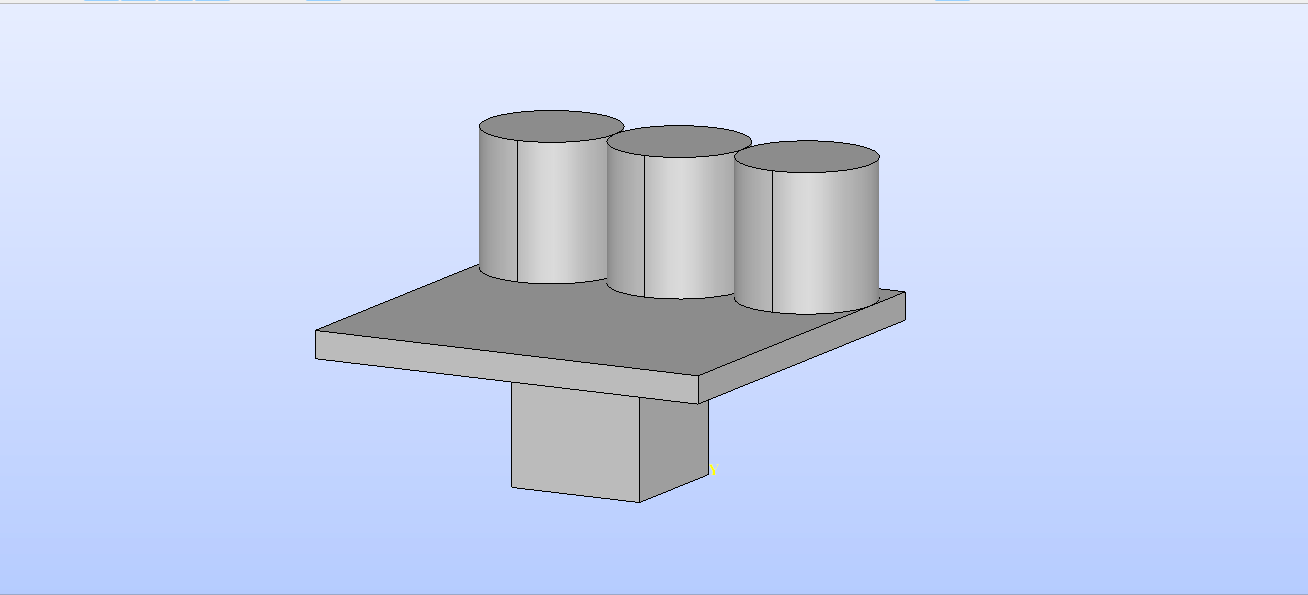
\includegraphics[width=0.5\linewidth]{1.1.png}
			\caption{Модель геометрии 1}
		\end{center}
	\end{figure}
	\begin{figure}[h]
		\begin{center}
			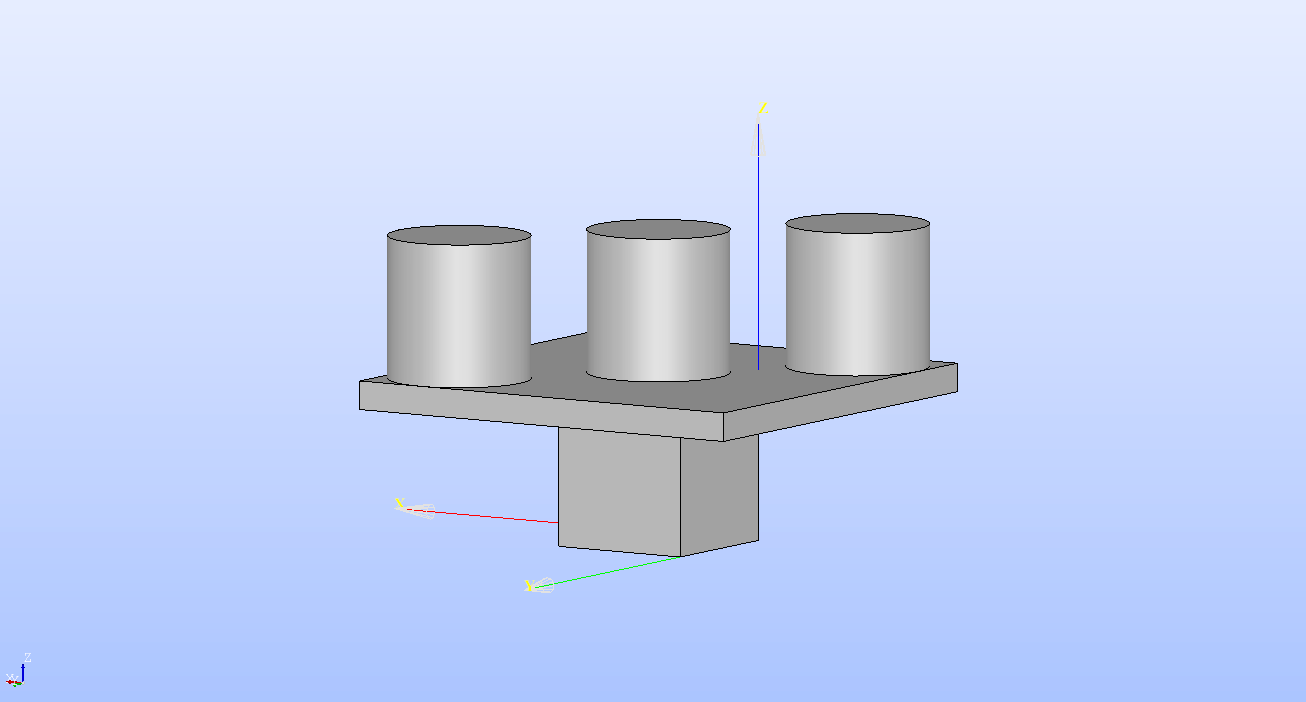
\includegraphics[width=0.5\linewidth]{1.2.png}
			\caption{Модель геометрии 2}
		\end{center}
	\end{figure}
\end{frame}

% Данные моделей и параметры задачи
\begin{frame}{Данные моделей и параметры задачи}
	\begin{table}[h]
		\begin{tabular}{|l|l|l|l|}
			\hline
			                                          & Нагреватель & Радиатор & Воздух        \\
			Плотность {[}кг/$м^3${]}                  & 1280        & 2700     & 1.196         \\
			\hline
			Cp   {[}Дж/кг*К{]}                        & 1004        & 900      & 1005          \\
			\hline
			Коэффициент теплопроводности {[}Вт/м*К{]} & 80          & 200      &               \\
			\hline
			Молекулярная масса {[}г/моль{]}           & 50          & 27       & 28.9          \\
			\hline
			Вязкость {[}кг/м*с{]}                     &             &          & $1.8*10^{-5}$ \\
			\hline
			Число Прандтля                            &             &          & 0.7           \\
			\hline
		\end{tabular}
		\caption{Параметры задачи} %% подпись к рисунку
	\end{table}
\end{frame}

% Графики результатов
\begin{frame}{Результаты}
	\begin{figure}[h]
		\begin{center}
			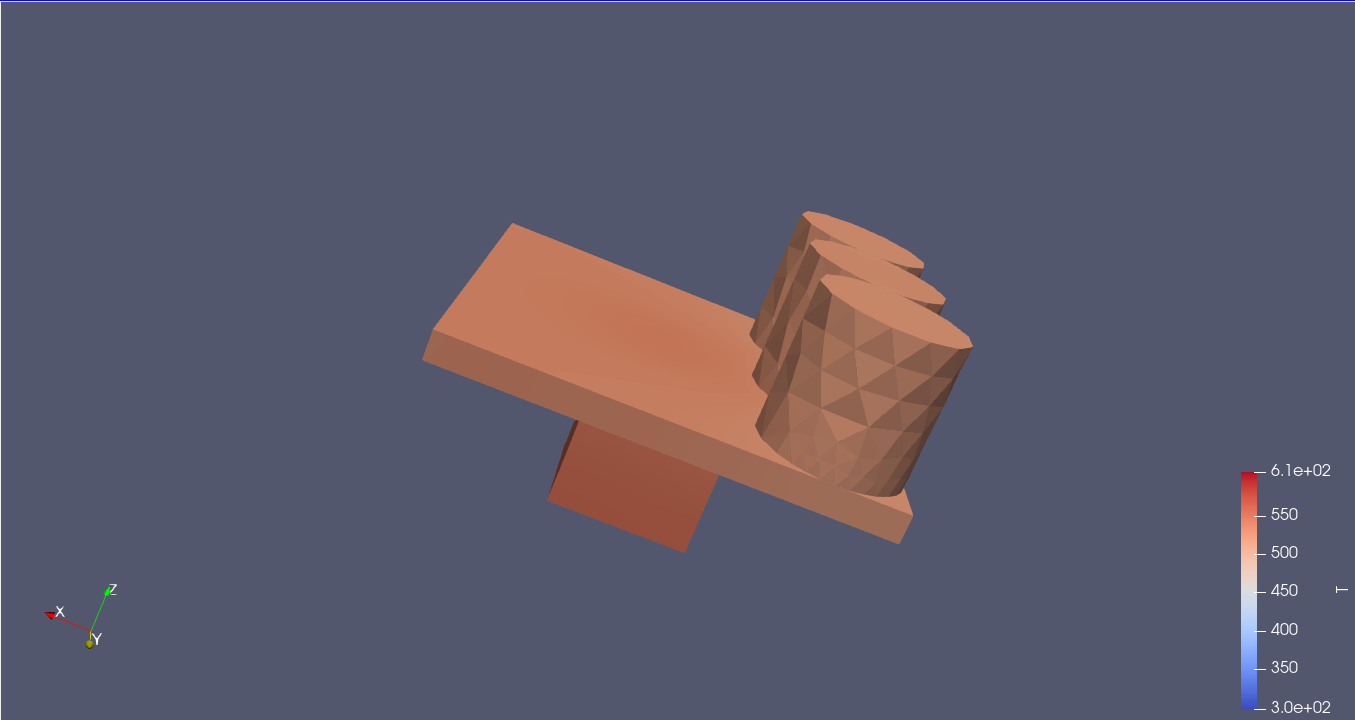
\includegraphics[width=0.45\linewidth]{5.1.png}
			\caption{Распределение температуры для модели 1}
		\end{center}
	\end{figure}
	\begin{figure}[h]
		\begin{center}
			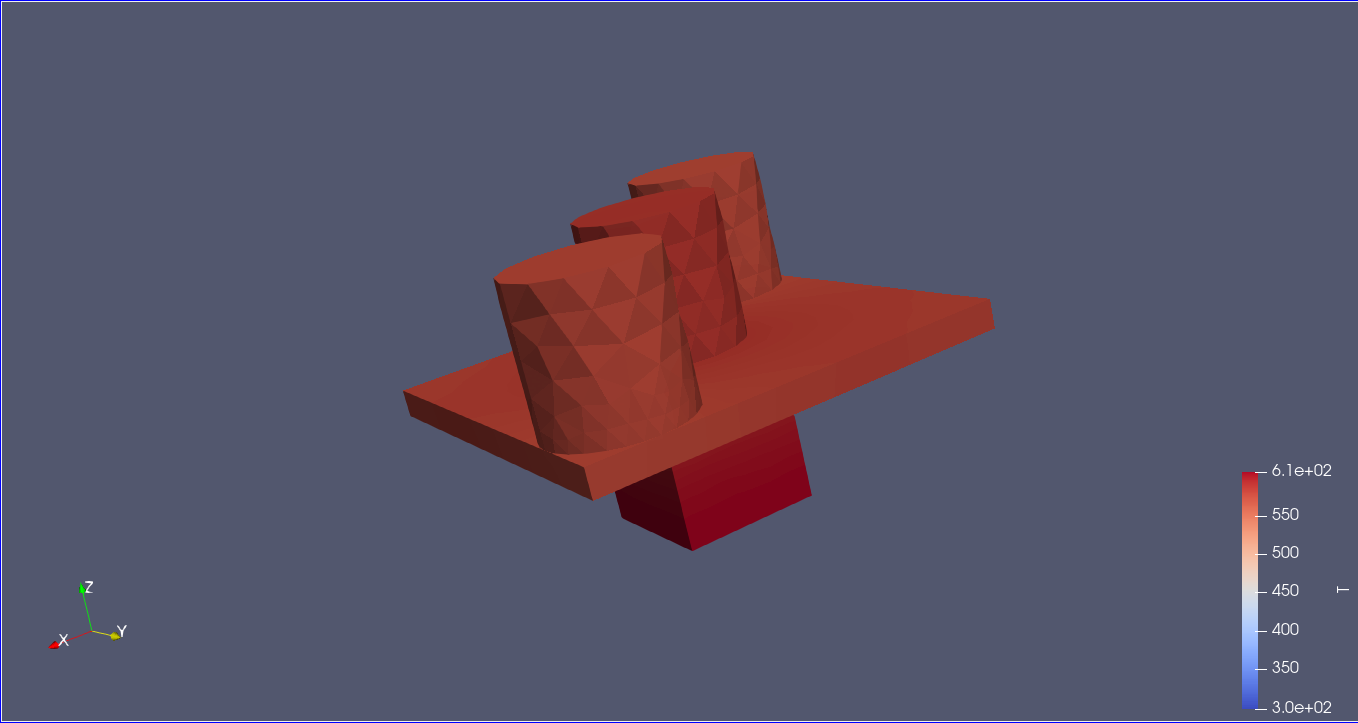
\includegraphics[width=0.45\linewidth]{5.2.png}
			\caption{Распределение температуры для модели 2}
		\end{center}
	\end{figure}
\end{frame}

\begin{frame}{Проблема с генерацией сетки в SALOME}
	В ходе исследования в SALOME возникли ошибки сетки из-за изменения идентификаторов форм при перегенерации геометрии. Решение было найдено с использованием Python API SALOME и следующих методов:

	\begin{itemize}[label=•]
		\item \textbf{SubShapeAllIDs:}
		      Получение всех идентификаторов подформ в геометрии.

		\item \textbf{GetShapesOnBoxIDs:}
		      Получение идентификаторов форм внутри заданного объема.

		\item \textbf{GetShapesOnPlaneWithLocationIDs:}
		      Получение идентификаторов форм, пересекаемых заданной плоскостью.
	\end{itemize}

	Эти методы стабилизировали процесс генерации сетки, обеспечив постоянство идентификаторов форм при обновлении геометрии, позволяя успешно использовать скрипт в дальнейших этапах исследования.
\end{frame}

\begin{frame}{Автоматизированный процесс: Параметры}
	На данном этапе рассматривается автоматизированный процесс генерации сетки в SALOME и расчетов в OpenFOAM с варьированием параметров.

	\begin{itemize}[label=•]
		\item \textbf{shift\_first\_cylinder:} Сдвиг первого цилиндра.
		\item \textbf{shift\_second\_cylinder:} Сдвиг второго цилиндра.
	\end{itemize}
\end{frame}

\begin{frame}{Автоматизированный процесс: Шаги}
	\begin{itemize}[label=•]
		\item Создание уникального имени для каждой комбинации параметров.
		\item Копирование исходного кейса в новую директорию.
		\item Запуск SALOME для генерации сетки с учетом новых параметров.
		\item Запуск bash-скриптов в OpenFOAM для выполнения кейса.
		\item Автоматическое извлечение результатов, включая данные теплообмена.
		\item Анализ влияния параметров на теплоотдачу системы.
	\end{itemize}
\end{frame}

\begin{frame}{Особенности фиксации и движения цилиндров}
	\begin{itemize}[label=•]
		\item В проведенных исследованиях использовались три цилиндра в системе.
		\item Третий цилиндр был зафиксирован в положении (0, 0).
		\item Двигались только два оставшихся цилиндра.
	\end{itemize}

	\vspace{1em}
	Такой подход облегчает визуализацию и анализ результатов, позволяя лучше понять влияние параметров на эффективность теплообмена в системе.
\end{frame}

\begin{frame}{Первые результаты}
	На основе автоматизированного процесса получены первые результаты, охватывающие 25 точек варьирования параметров.

	\vspace{1em}
	\begin{itemize}
		\item Исследуемые параметры: \texttt{shift\_first\_cylinder} и \texttt{shift\_second\_cylinder}.
		\item Изменялись от 0 до 20 с шагом 5.
	\end{itemize}

	\begin{figure}[h]
		\centering
		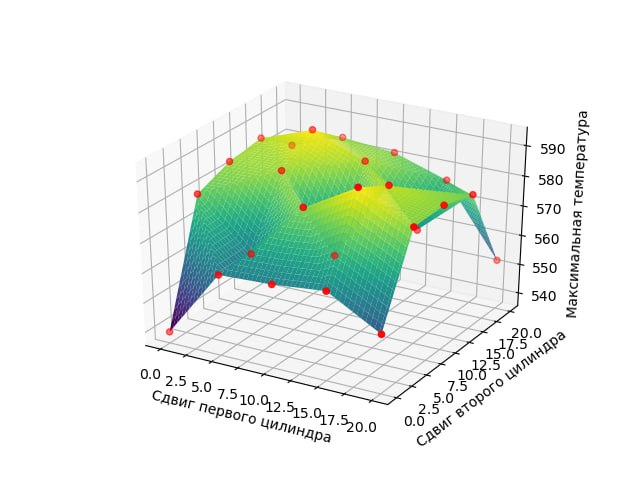
\includegraphics[width=0.4\linewidth]{16.1.jpg}
		\caption{Зависимость максимальной температуры нагревателя от сдвигов цилиндров}
	\end{figure}

	\begin{figure}[h]
		\centering
		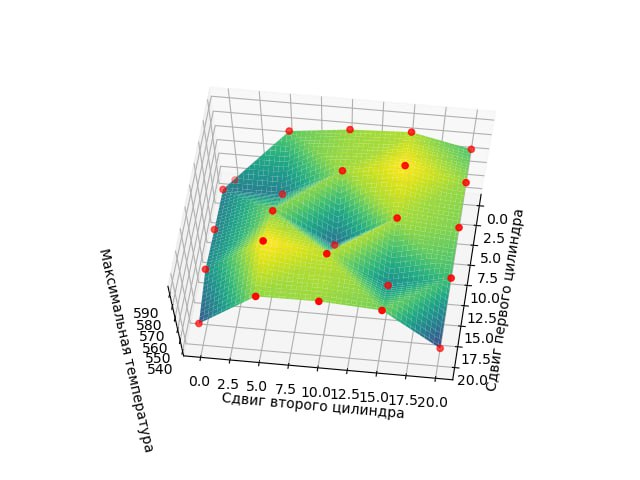
\includegraphics[width=0.4\linewidth]{16.2.jpg}
		\caption{Зависимость максимальной температуры нагревателя от сдвигов цилиндров}
	\end{figure}
\end{frame}

\begin{frame}{Первые результаты (продолжение)}
	\begin{figure}[h]
		\centering
		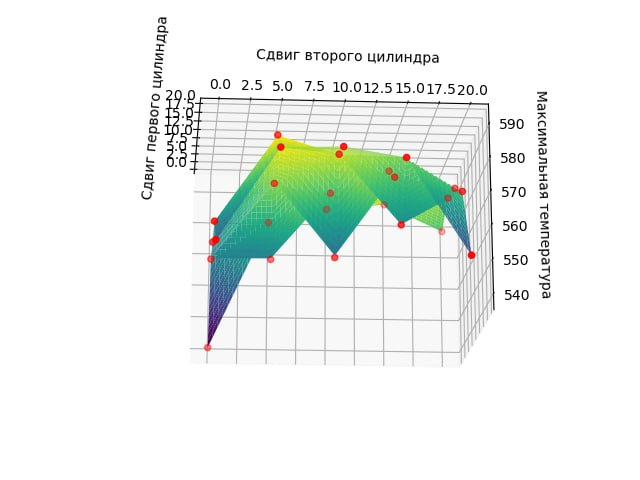
\includegraphics[width=0.4\linewidth]{16.3.jpg}
		\caption{Зависимость максимальной температуры нагревателя от сдвигов цилиндров}
	\end{figure}

	\vspace{1em}
	Для улучшения визуализации и наглядности данных была проведена интерполяция поверхности. Интерполированная поверхность дает представление о поведении системы в пространстве параметров и позволяет выявить области оптимальных значений для исследуемых параметров.

	\vspace{1em}
	Этот этап анализа предоставляет первичное представление о влиянии сдвига цилиндров на теплообмен в системе.
\end{frame}

\begin{frame}{Оптимизация процесса расчета}
	С целью оптимизации процесса расчета для большего количества точек был реализован многопоточный код на языке программирования Python с использованием модуля \texttt{multiprocessing}.

	\vspace{1em}
	\begin{itemize}
		\item Внесены изменения в код для поддержки третьего цилиндра (\texttt{shift\_third\_cylinder}) и сбора результатов в разделяемом словаре (\texttt{all\_data}).
		\item Реализована функция \texttt{run\_simulation}, выполняющая расчет для каждой комбинации параметров в отдельном процессе.
		\item Результаты сохраняются в разделяемом словаре, где ключи - уникальные идентификаторы, значения - результаты расчетов.
		\item Применена библиотека Pool и метод \texttt{starmap} для распараллеливания выполнения расчетов.
	\end{itemize}

	\vspace{1em}
	Итоги расчетов собраны в разделяемом словаре \texttt{all\_data}, что позволяет эффективно обрабатывать большой объем данных при анализе.
\end{frame}

\begin{frame}{Первые результаты и наблюдения}
	Первые результаты анализа геометрии системы показали интересные закономерности.

	\vspace{1em}
	\begin{itemize}
		\item Минимумы характеристик системы наблюдаются при равных сдвигах первого и второго цилиндров.
	\end{itemize}

	\begin{figure}[h]
		\centering
		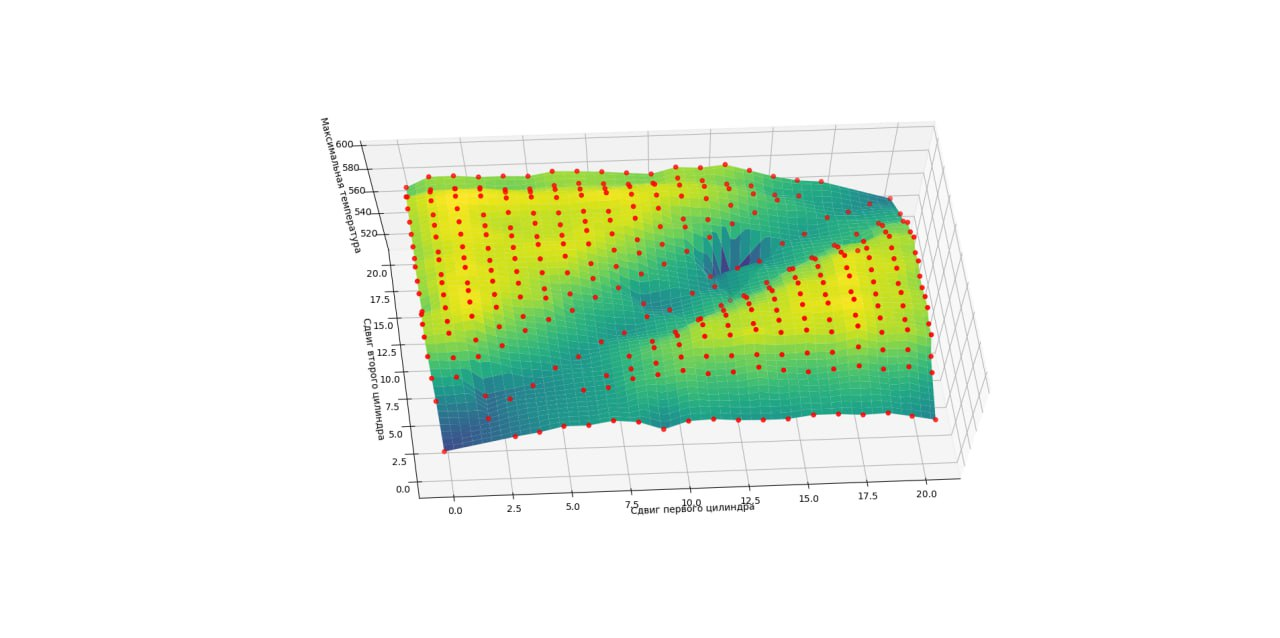
\includegraphics[width=0.4\linewidth]{18.3.jpg}
		\caption{Зависимость максимальной температуры нагревателя от сдвигов цилиндров (441 точка)}
	\end{figure}

	При равных сдвигах цилиндров они касаются друг друга, способствуя более эффективному теплообмену и равномерному распределению тепловой нагрузки.

	\begin{figure}[h]
		\centering
		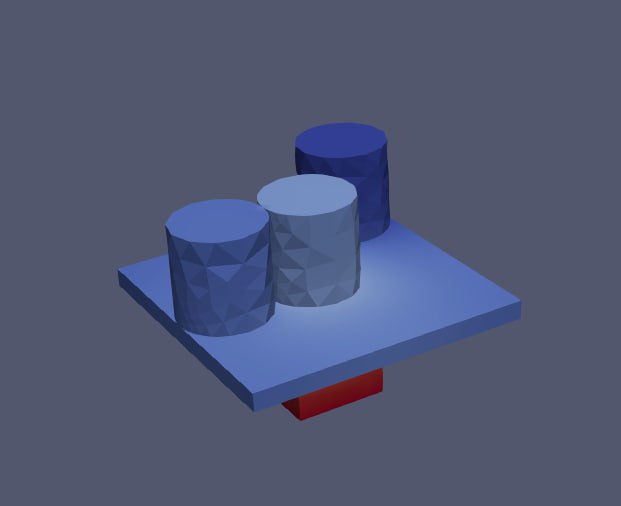
\includegraphics[width=0.4\linewidth]{19.jpg}
		\caption{Геометрия, при которой достигается минимальное значение}
	\end{figure}
\end{frame}

\begin{frame}{Эксперименты с геометрией и анализ результатов}
	Однако эта геометрия не демонстрировала реальной зависимости между расположением цилиндров и температурой. В ответ на это наблюдение был проведен ряд экспериментов с общей геометрией системы.

	\begin{figure}[h]
		\centering
		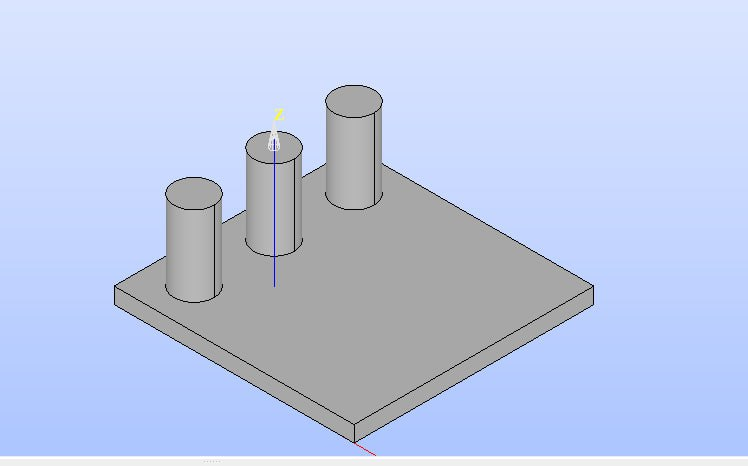
\includegraphics[width=0.4\linewidth]{20.jpg}
		\caption{Новая геометрия}
	\end{figure}

	После внесения изменений в геометрию системы были получены более интересные результаты.

	\begin{figure}[h]
		\centering
		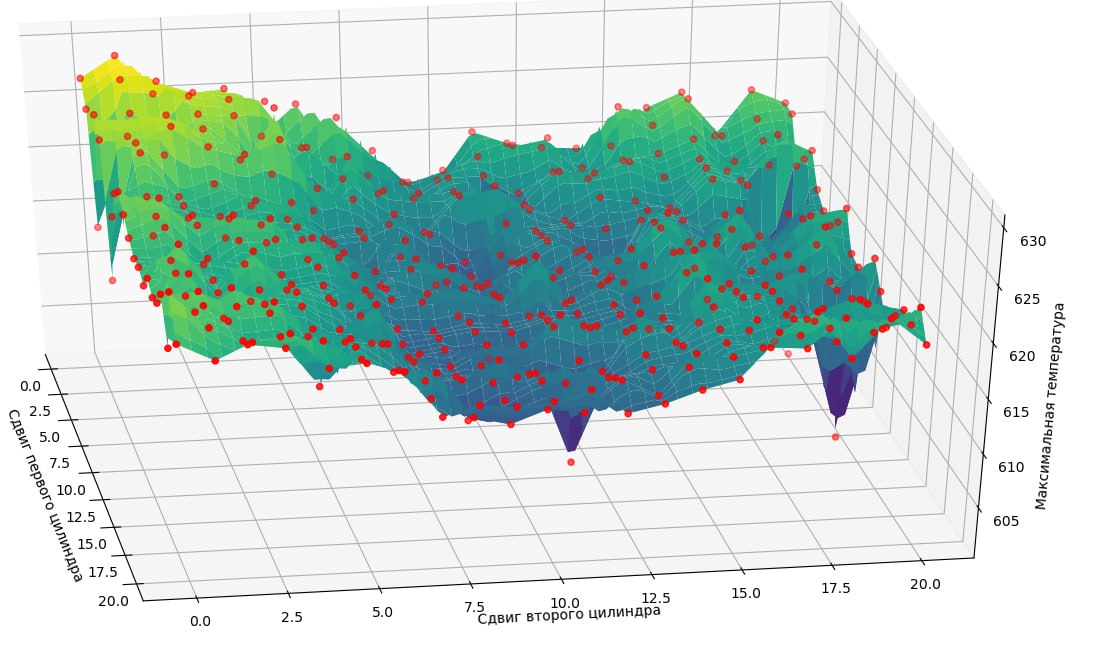
\includegraphics[width=0.4\linewidth]{21.1.jpg}
		\caption{Зависимость максимальной температуры нагревателя от сдвигов цилиндров}
	\end{figure}
	\begin{figure}[h]
		\centering
		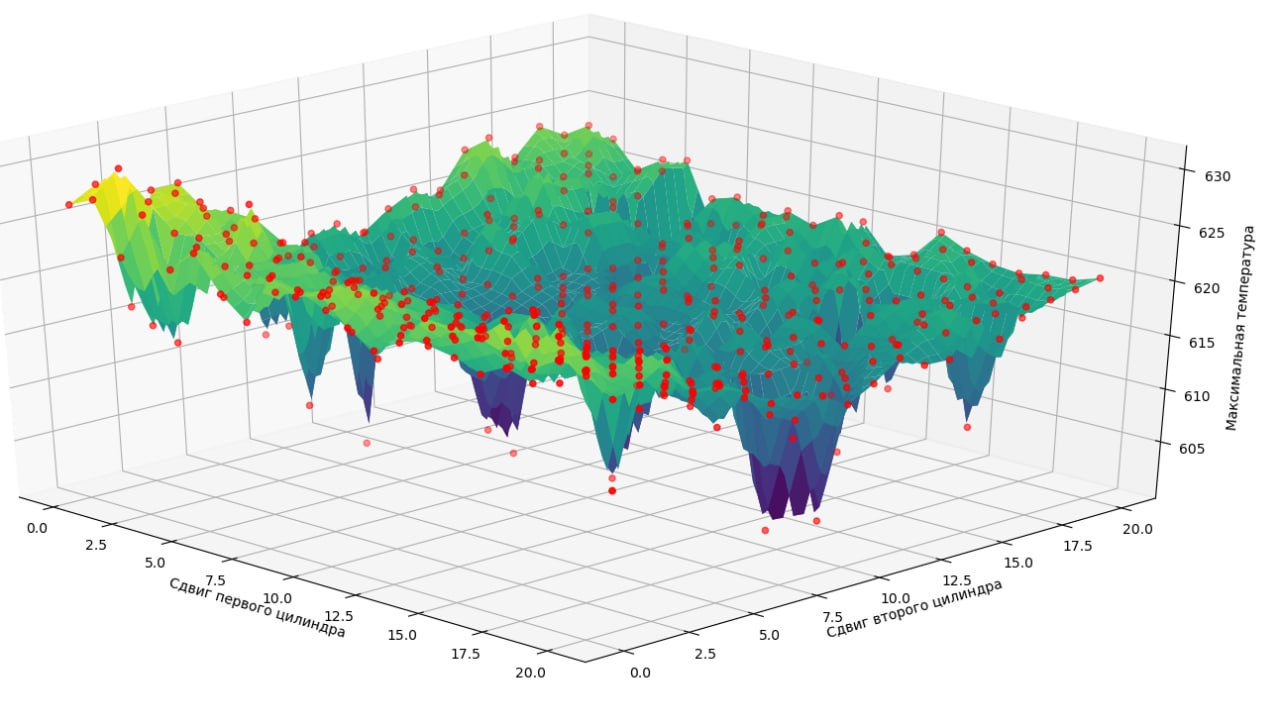
\includegraphics[width=0.4\linewidth]{21.2.jpg}
		\caption{Зависимость максимальной температуры нагревателя от сдвигов цилиндров}
	\end{figure}
	\begin{figure}[h]
		\centering
		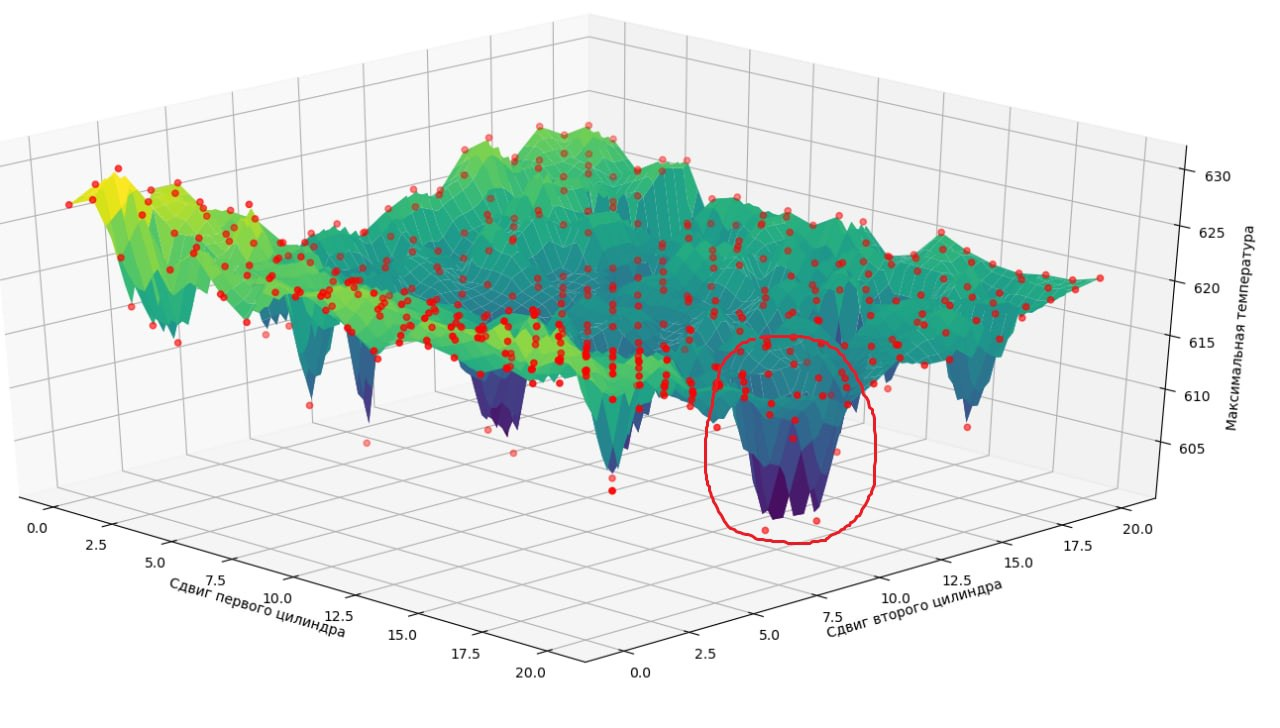
\includegraphics[width=0.4\linewidth]{21.3.jpg}
		\caption{Зависимость максимальной температуры нагревателя от сдвигов цилиндров}
	\end{figure}

	В ходе экспериментов было обнаружено, что существует оптимальная конфигурация, при которой достигается минимум температуры в системе.

	\begin{figure}[h]
		\centering
		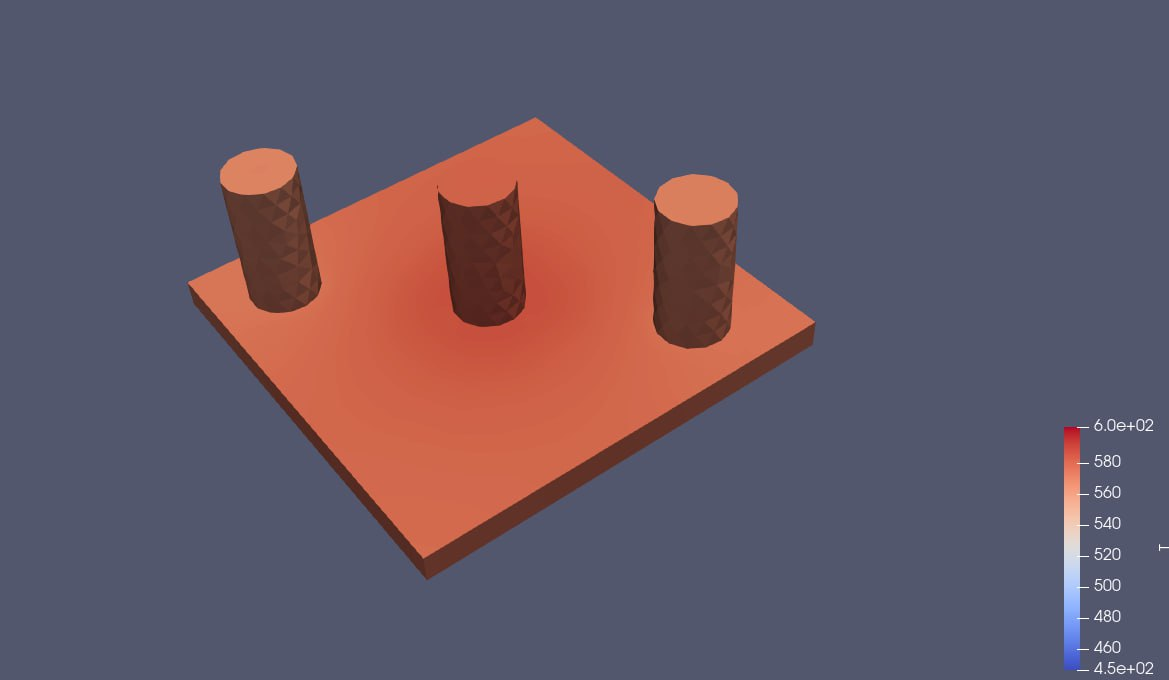
\includegraphics[width=0.4\linewidth]{21.4.jpg}
		\caption{Пример минимума при новой геометрии}
	\end{figure}
\end{frame}

\begin{frame}{Эксперименты с геометрией и анализ результатов (продолжение)}
	\begin{figure}[h]
		\centering
		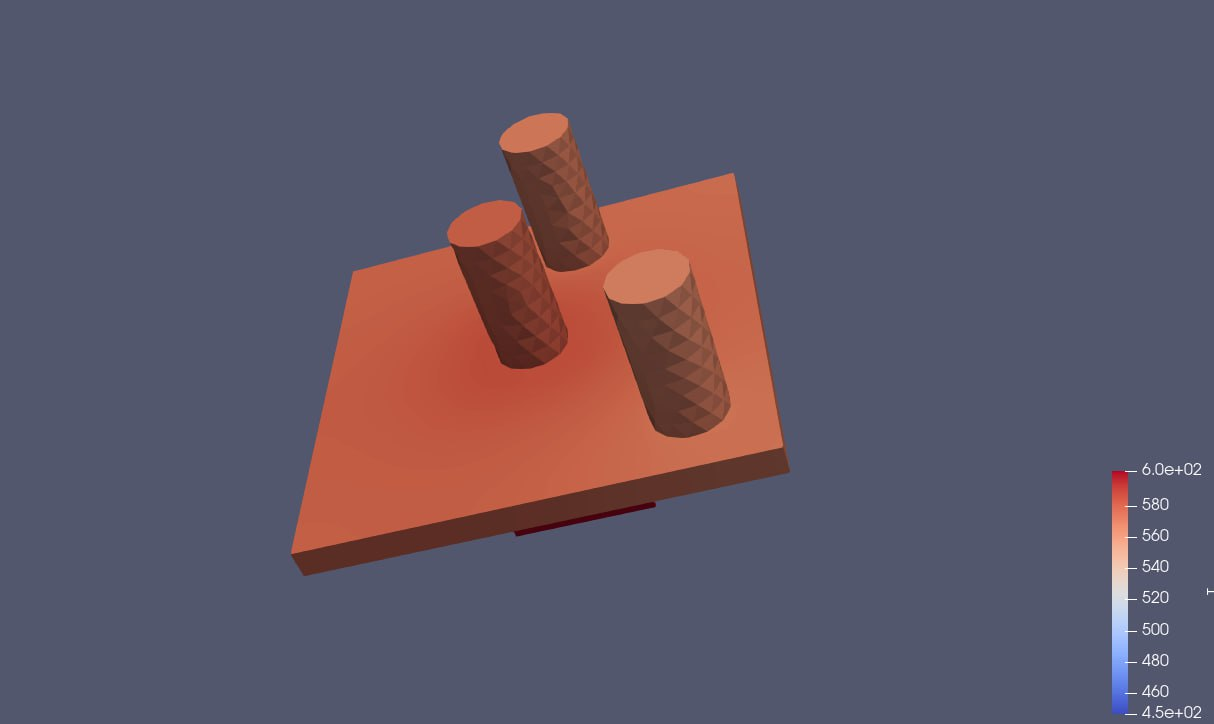
\includegraphics[width=0.4\linewidth]{21.5.jpg}
		\caption{Пример минимума при новой геометрии}
	\end{figure}

	Эта конфигурация характеризуется расстановкой цилиндров по диагонали.

	\vspace{1em}
	\begin{itemize}
		\item Минимум максимальной температуры нагревателя также достигается при данной конфигурации.
	\end{itemize}
\end{frame}

\begin{frame}{Анализ реальной системы и изменения параметров}
	Следующим этапом исследования стал анализ условий, представляющих реальную систему охлаждения. Внесенные изменения включали снижение скорости воздуха внутри воздуховода до 3 м/с (по сравнению с предыдущим значением 5.6 м/с), замену материала радиатора на медь (предыдущий материал - алюминий), а также модификацию геометрии нагревателя, сделав его тоньше и значительно больше по размерам, а саму подложку радиатора сделав толще.

	\begin{figure}[h]
		\centering
		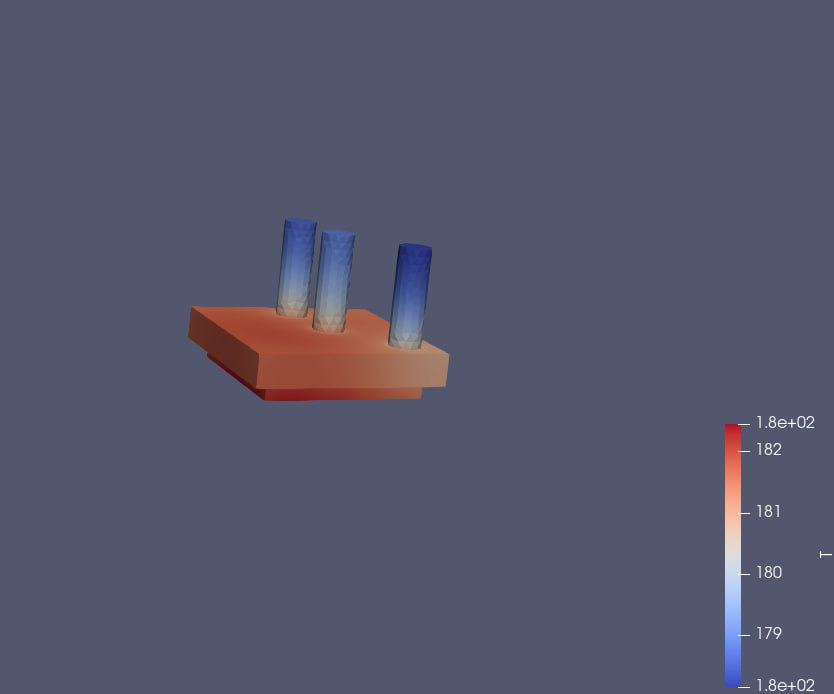
\includegraphics[width=0.4\linewidth]{23.1.jpg}
		\caption{Измененная геометрия}
	\end{figure}
	\begin{figure}[h]
		\centering
		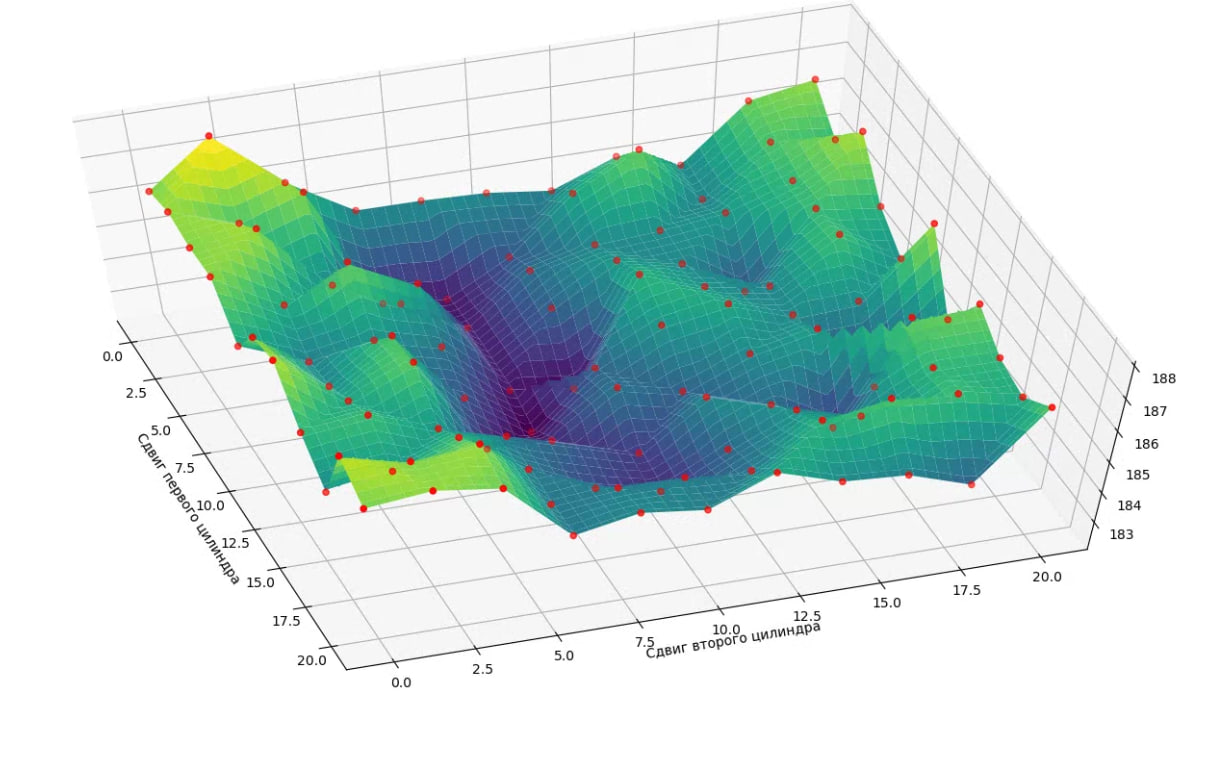
\includegraphics[width=0.4\linewidth]{23.2.jpg}
		\caption{Зависимость максимальной температуры нагревателя от сдвигов цилиндров}
	\end{figure}
	\begin{figure}[h]
		\centering
		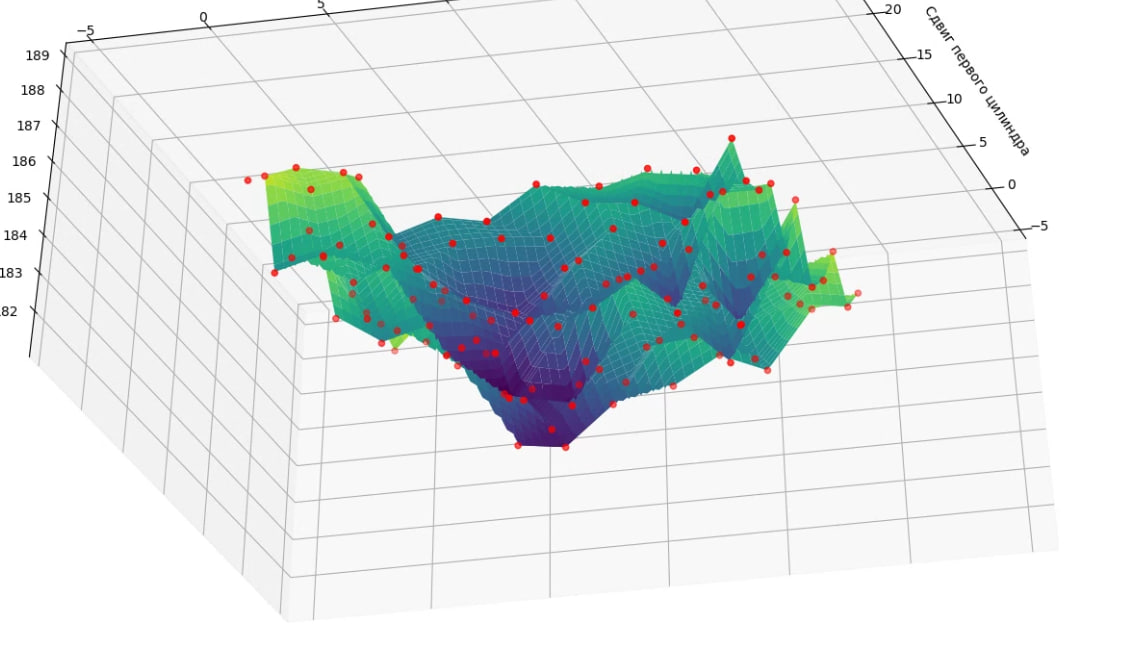
\includegraphics[width=0.4\linewidth]{23.3.jpg}
		\caption{Зависимость максимальной температуры нагревателя от сдвигов цилиндров}
	\end{figure}
\end{frame}

\begin{frame}{Применение эволюционного алгоритма в оптимизации}
	Необходимо отметить, что для более эффективного и быстрого поиска оптимальных параметров в задаче охлаждения был применен эволюционный алгоритм.

	\begin{itemize}
		\item \textbf{Инициализация популяции:} Создается начальная популяция индивидов (наборов параметров) случайным образом или на основе каких-то эвристик.

		\item \textbf{Оценка приспособленности:} Каждый индивид из популяции оценивается по степени приспособленности в соответствии с целевой функцией.

		\item \textbf{Отбор:} Выбираются наиболее приспособленные индивиды для следующего поколения.

		\item \textbf{Скрещивание:} Происходит кроссовер (скрещивание) между выбранными индивидами, что приводит к созданию новых индивидов.

		\item \textbf{Мутация:} Некоторые индивиды могут подвергаться мутациям, изменяя свои параметры с определенной вероятностью.

		\item \textbf{Повторение:} Описанные шаги повторяются в цикле до достижения критерия остановки, такого как заданное количество поколений или достижение требуемой точности.
	\end{itemize}

	Применение эволюционного алгоритма существенно ускорило поиск оптимальных параметров в условиях ограниченной информации о системе \cite{evolution}.
\end{frame}

\begin{frame}{Использование градиентного метода}

	Помимо дифференциальной эволюции, данная работа включала использование градиентного метода для оптимизации. Градиентные методы широко используются в численной оптимизации для поиска минимума (или максимума) функции. Один из простых градиентных методов - это метод градиентного спуска.

	% \begin{enumerate}
	% 	\item Инициализация параметров случайными значениями.
	% 	\item Повторение до сходимости (или до достижения максимального числа итераций):
	% 	      \begin{itemize}
	% 		      \item Вычисление градиента функции по параметрам.
	% 		      \item Обновление параметров в направлении, противоположном градиенту.
	% 	      \end{itemize}
	% \end{enumerate}

	% Однако метод градиентного спуска может иметь ограничения, такие как сходимость к локальным минимумам или чувствительность к выбору начальных значений параметров \cite{Chernyshev2007}.

	% \begin{figure}[h]
	% 	\centering
	% 	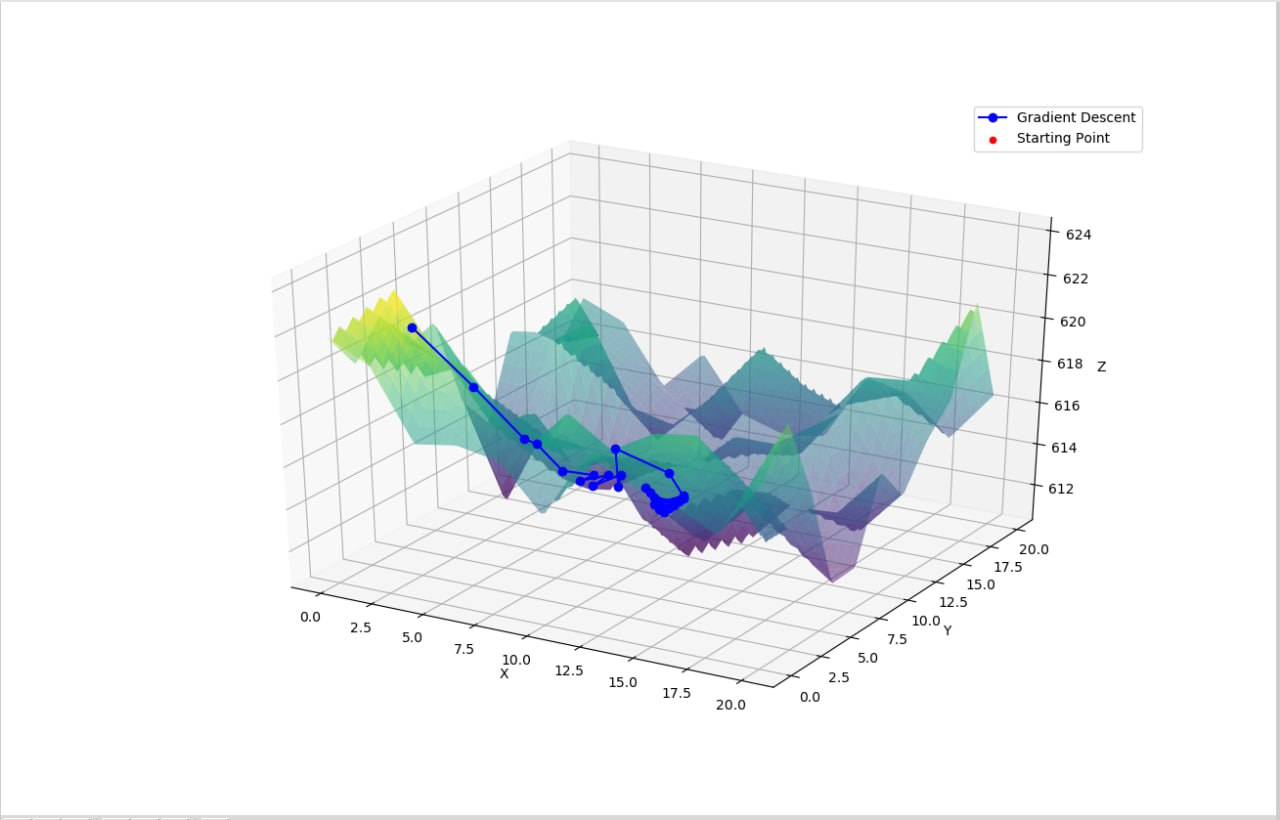
\includegraphics[width=0.4\linewidth]{24.jpg}
	% 	\caption{Зависимость максимальной температуры нагревателя от сдвигов цилиндров}
	% \end{figure}
\end{frame}

\begin{frame}{Использование L-BFGS-B в оптимизации}

	\textbf{L-BFGS-B (Limited-memory Broyden-Fletcher-Goldfarb-Shanno with Bound constraints):}

	L-BFGS-B - это усовершенствованный метод оптимизации, предназначенный для решения задач с ограничениями. Он поддерживает локальную оптимизацию с ограничениями на параметры.

	% \begin{enumerate}
	% 	\item Ограничения:
	% 	      \begin{itemize}
	% 		      \item Метод позволяет оптимизировать функцию с учетом границ (ограничений) для параметров. Это важно, когда некоторые параметры должны оставаться в пределах определенных значений.
	% 	      \end{itemize}
	% 	\item Лимит памяти:
	% 	      \begin{itemize}
	% 		      \item "Limited-memory" в названии относится к тому, что метод хранит ограниченное количество предыдущих итераций для оценки гессиана. Это особенно полезно, когда размерность пространства параметров велика.
	% 	      \end{itemize}
	% 	\item BFGS-подобные обновления:
	% 	      \begin{itemize}
	% 		      \item Метод L-BFGS-B использует обновления BFGS для оценки обратного гессиана, что позволяет улучшить сходимость метода.
	% 	      \end{itemize}
	% \end{enumerate}

	% Использование L-BFGS-B может быть предпочтительным, особенно при наличии ограничений на параметры. Этот метод часто применяется в задачах оптимизации, таких как подгонка параметров в статистических моделях или решение задач машинного обучения, где требуется минимизация функции потерь \cite{limited_BFGS}.
\end{frame}

\begin{frame}{Заключение}

	В ходе данной работы было проведено комплексное исследование системы охлаждения с использованием численных методов и оптимизации. Основные выводы и результаты работы:

	% \begin{enumerate}
	% 	\item \textbf{Геометрические изменения:} проведен анализ геометрии системы, выполнено исследование влияния расположения цилиндров на эффективность охлаждения. Эксперименты с различными конфигурациями позволили выявить оптимальные расстановки и влияние контакта цилиндров друг с другом на тепловые характеристики.

	% 	\item \textbf{Оптимизация с использованием полного перебора:} проведена первоначальная оптимизация системы, использован полный перебор, что позволило выявить оптимальные точки в пространстве параметров. Это дало общий обзор зависимостей и минимумов целевой функции.

	% 	\item \textbf{Многопоточность для улучшения производительности:} в процессе увеличения количества точек в пространстве параметров использовалась многопоточность для оптимизации, что значительно ускорило процесс расчета и позволило нам провести более подробное исследование.

	% 	\item \textbf{Изменения в геометрии и параметрах системы:}исследовали влияние различных параметров, таких как скорость воздуха и материалы, на эффективность охлаждения. Изменения в геометрии и параметрах системы привели к новым интересным результатам, позволяя лучше понять зависимости и оптимизировать систему.

	% 	\item \textbf{Эволюционный алгоритм:} применили эволюцион

	% 	      ный алгоритм для оптимизации системы. Этот метод позволил более эффективно находить точки минимума, снижая количество расчетов по сравнению с полным перебором.

	% 	\item \textbf{Градиентные методы оптимизации:} использование градиентных методов, таких как L-BFGS-B, добавило эффективность и точность в арсенал оптимизационных методов.

	% 	\item \textbf{Выводы и перспективы:} на основе результатов исследования необходимо сделать вывод о том, что оптимизация геометрии и параметров системы охлаждения может существенно повысить ее эффективность. Подход с использованием различных методов оптимизации и численного моделирования предоставляет мощный инструментарий для разработки и улучшения теплоотводящих систем. В будущем возможно проведение более глубоких исследований с учетом дополнительных факторов и условий эксплуатации системы.
	% \end{enumerate}
\end{frame}

\end{document}